\documentclass[newstyle]{cotesysposter}

\usepackage{graphicx}
\usepackage{amsmath}
\usepackage{wrapfig}
\usepackage{url}
\usepackage{iasbib}
\usepackage{bm}
\usepackage{amssymb}

\usepackage{tikz}
\usepackage{pgfmoreshapes}
\usetikzlibrary{arrows,shapes,er}


\graphicspath{{../../../pictures/src/}}
%\usepackage[ansinew]{inputenc} % Activate Support for Umlaute

\newenvironment{Code}[0]{\scriptsize
                         \begin{tabbing}
                         \hspace*{2ex}\=\hspace*{2ex}\=\hspace*{2ex}\=\hspace*{2ex}\=\kill}%
                        {\end{tabbing}}
\newcommand{\kw}[1]{\textbf{#1}}

\definecolor{alertcolor}{HTML}{E4111F}

\title{Voxelized Shape and Color Histograms for RGB-D}
\author{Asako Kanezaki, Zoltan-Csaba Marton, Dejan Pangercic, Tatsuya Harada, Yasuo Kuniyoshi, and Michael Beetz}
\email{\normalsize\{kanezaki, harada, kuniyosh\}@isi.imi.i.u-tokyo.ac.jp, \{marton, pangercic, beetz\}@cs.tum.edu}
\homepage{http://www.isi.imi.i.u-tokyo.ac.jp}
\homepage{http://ias.cs.tum.edu}
\group{Intelligent Systems and Informatics Lab.}
\university{The University of Tokyo, Japan}
\group{Intelligent Autonomous Systems}
\university{Technische Universit\"at M\"unchen, Munich, Germany}

% \newcommand{\code}[1]{\texttt{#1}}
% \newcommand{\texcode}[1]{\texttt{\textbackslash#1}}
% \newcommand{\texcmd}[2]{\texttt{\textbackslash#1\{#2\}}}
% \newcommand{\texcmdd}[3]{\texttt{\textbackslash#1\{#2\}\{#3\}}}

\newcommand{\mtext}[1]{\textit{#1}}

\begin{document}

\posterboxroundnessstandard
\posterbox[Motivation]{

%\begin{wrapfigure}[]{r}{0.5\columnwidth}
 %\vspace{-1em}

% \includegraphics[width=0.5\columnwidth]{cotesys/10_fall_workshop/demo_3_crop_persp.jpg}
% \includegraphics[width=0.40\columnwidth]{cogman/pancake/pancake_err_3.jpg}
%\end{wrapfigure}

  \begin{wrapfigure}[]{r}{0.35\columnwidth}
    \centering
    \vspace{-4ex}
    \includegraphics[width=0.35\columnwidth]%
    {../figures/firstpage/firstpage.pdf}\\
    % {knowledge/ehow/make_pancakes.png}\\
    \includegraphics[width=0.35\columnwidth]%
    {../figures/objects/objects_s.jpg}\\
     \vspace{2ex}
  \end{wrapfigure}

  One of the great challenges in autonomous mobile robot manipulation is scaling
  technology to realistic tasks in real-world environments and conditions.
  Real world environments typically include objects with different perceptual appearances, that is,
  \emph{textured, textureless} and even partially transparent objects.
  While perception methods exist that work well on one such class of objects at a time, the perception of
  various classes of objects in a scene is still a challenge.

  \vspace{2ex}
    
  We present an approach that enables efficiently capturing both the geometric
  and visual appearance of common objects of daily use.

}

\vfill

\posterbox[Proposed Approach]{

  \begin{itemize}
  \item Developed \emph{\textbf{ConVOSCH}} and \emph{\textbf{VOSCH}} descriptors based on C$^3$-HLAC and GRSD
  \item Acquired the training data for 63 objects of daily use using the \emph{\textbf{Kinect sensor}}

  \item Generated training models using Support Vector Machines (SVM) or Linear \\ Subspace Method (LSM) classifiers
  \end{itemize}

  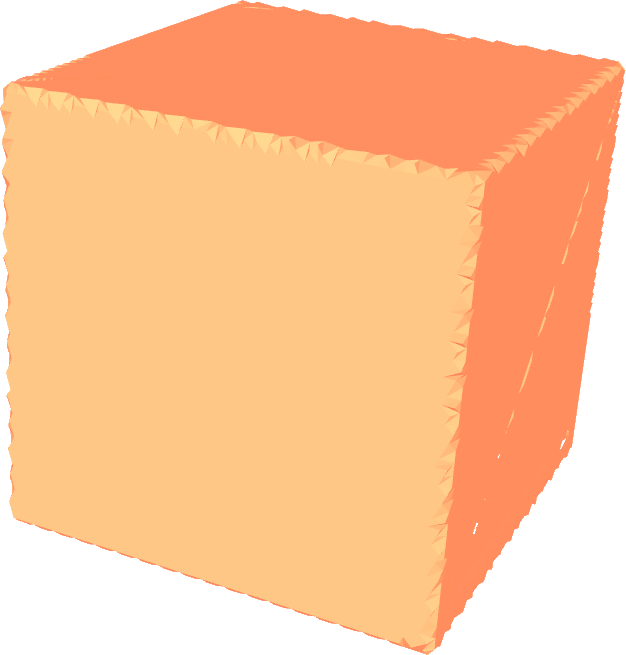
\includegraphics[width=.14\columnwidth]{../figures/comparison/cube.png}
  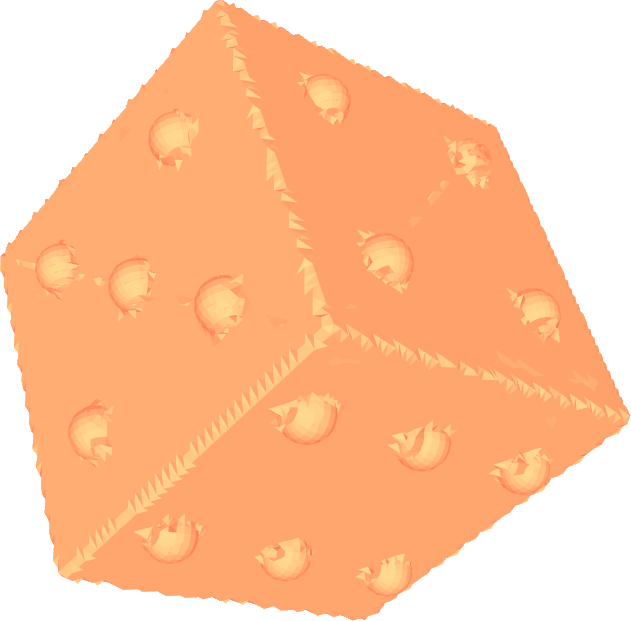
\includegraphics[width=.16\columnwidth]{../figures/comparison/dice1.png}
  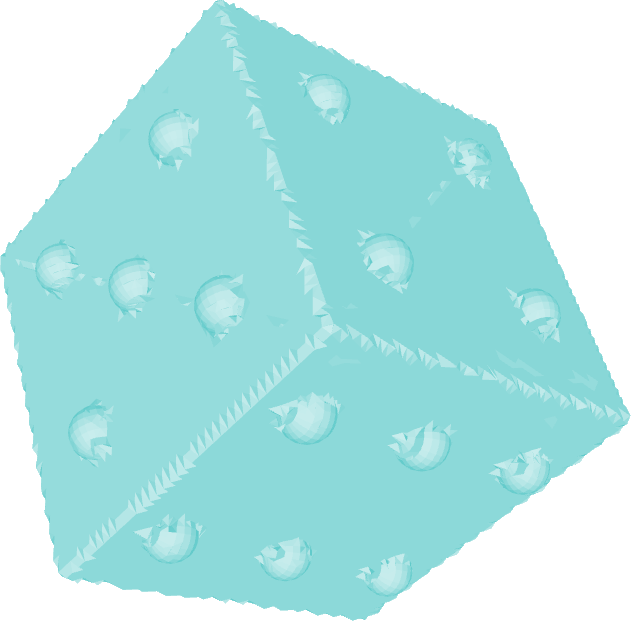
\includegraphics[width=.16\columnwidth]{../figures/comparison/dice2.png}
  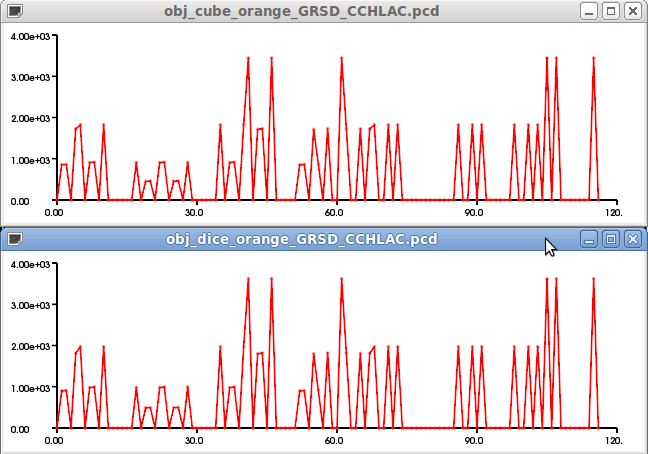
\includegraphics[width=.22\columnwidth]{../figures/comparison/orange_cube_vs_orange_dice.png}
  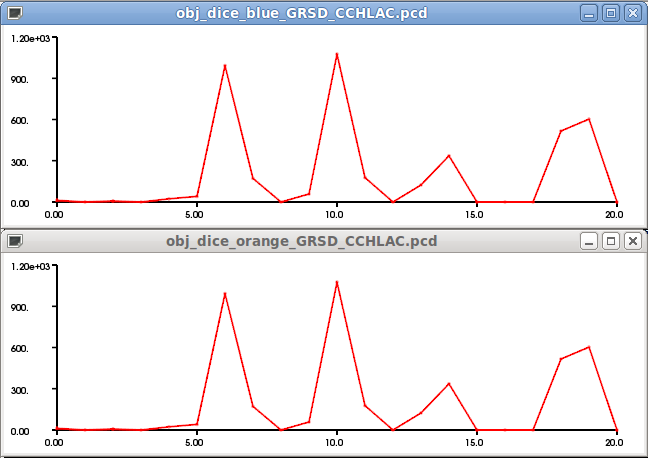
\includegraphics[width=.22\columnwidth]{../figures/comparison/blue_vs_orange_dice_grsd.png}


%%   \textbf{Contributions:}

%%   \begin{itemize}
%%   \item Novel descriptor that account for geometrical and visual appearance properties
%%   \item An extensive database of 63 objects of daily use captured with the Kinect sensor
%%   \item A comparison of classification results for SVM and LSM
%%   \end{itemize}

}

\vfill


\posterboxroundnessstandard
\posterbox[C$^3$-HLAC]{

  Circular Color Cubic Higher-order Local Auto-Correlation descriptor (C$^3$-HLAC~\cite{kanezaki2011icra}) descriptor
  is a high-dimensional vector that measures the summation of the 
  multiplied RGB values of neighboring voxels in a $3 \times 3 \times 3$ grid around a voxel grid of arbitrary size. 
  When $p({\bm x})\hspace{-1mm}=\hspace{-1mm}1 $, 
  a voxel status $\bm{f}(\bm{x})\in \mathbb{N}^6$ is defined as $\left[r_1({\bm x})\hspace{1.5mm} r_2(\bm{x}) \hspace{1.5mm}g_1({\bm x}) \hspace{1.5mm}g_2({\bm x}) \hspace{1.5mm}b_1({\bm x}) \hspace{1.5mm}b_2({\bm x})\right]^T $, 
  or a zero vector, otherwize.

  \begin{itemize}
  \item $\bm{x}=(x,y,z)^T$ : the position of a voxel
  \item $p(\bm{x})$ : the flag for occupancy of the voxel
  \item $r(\bm{x})$, $g(\bm{x})$ and $b(\bm{x})$ : normalized RGB values
  \item $r_1(\bm{x}) \equiv sin\left( \frac{\pi}{2}r(\bm{x})\right)$, $g_1(\bm{x}) \equiv sin\left( \frac{\pi}{2}g(\bm{x})\right)$, $b_1(\bm{x}) \equiv sin\left( \frac{\pi}{2}b(\bm{x})\right)$, 
  \item $r_2(\bm{x}) \equiv cos\left( \frac{\pi}{2}r(\bm{x})\right)$, $g_2(\bm{x}) \equiv cos\left( \frac{\pi}{2}g(\bm{x})\right)$, and $b_2(\bm{x}) \equiv cos\left( \frac{\pi}{2}b(\bm{x})\right)$, 
  \end{itemize}

  \vspace{1ex}

  Letting ${\bm a_i}$ be a displacement vector from the reference voxel to its neighboring voxel, 
  a C$^3$-HLAC descriptor extracted from a voxel grid $V$ are calculated by the following:
  \begin{equation}\label{eq:0th}
    {\bm q_1} = \sum_{{\bm x} \in V} \bm{f}({\bm x})
  \end{equation}
  \vspace{-2mm}
  \begin{equation}\label{eq:0th_1}
    {\bm q_2} = \sum_{{\bm x} \in V} \bm{f}({\bm x}) \hspace{1mm}\bm{f}^T({\bm x}) \\
  \end{equation}
  \vspace{-2mm}
  \begin{equation}\label{eq:1st}
    {\bm q_3}({\bm a}_i) = \sum_{{\bm x} \in V} \bm{f}({\bm x}) \hspace{1mm}\bm{f}^T({\bm x}+{\bm a_i}) \;\;\; (i=0, \dots 12) \\
  \end{equation}
}

\posterboxroundnessstandard
\posterbox[GRSD]{

Global Radius-based Surface Descriptor (GRSD~\cite{GRSD10Humanoids}) is a histogram, that counts the number of transitions between different types of voxels.
We used it to count the transitions between the following geometric classes of voxel surfaces: \emph{free space, plane, cylinder, sphere, rim, and noise}.
Surface types were identified based on the estimation of their
two principal curves' radii, $r_{min}$ and $r_{max}$.
The number of bins $b$ is:
\begin{equation}
b=\frac{s(s+1)}{2}
\end{equation}
where $s$ is the number of possible surface types,
resulting in 21 dimensions for the above stated 6 types of surfaces.

}

\posterboxroundnessstandard
\posterbox[VOSCH]{
  \begin{itemize}
    \item \textbf{\emph{ConVOSCH}} is a mere concatenation of GRSD and C$^3$-HLAC histograms.
    \item \textbf{\emph{VOSCH}} is a concatenation of GRSD and rotation-invariant C$^3$-HLAC.
    \item To make C$^3$-HLAC rotation-invariant, we brought all 13 different vectors \\ given by (\ref{eq:1st}) together.
    \item GRSD was altered to have additive property, to efficiently merge the two features.
  \end{itemize}

  \begin{center}
    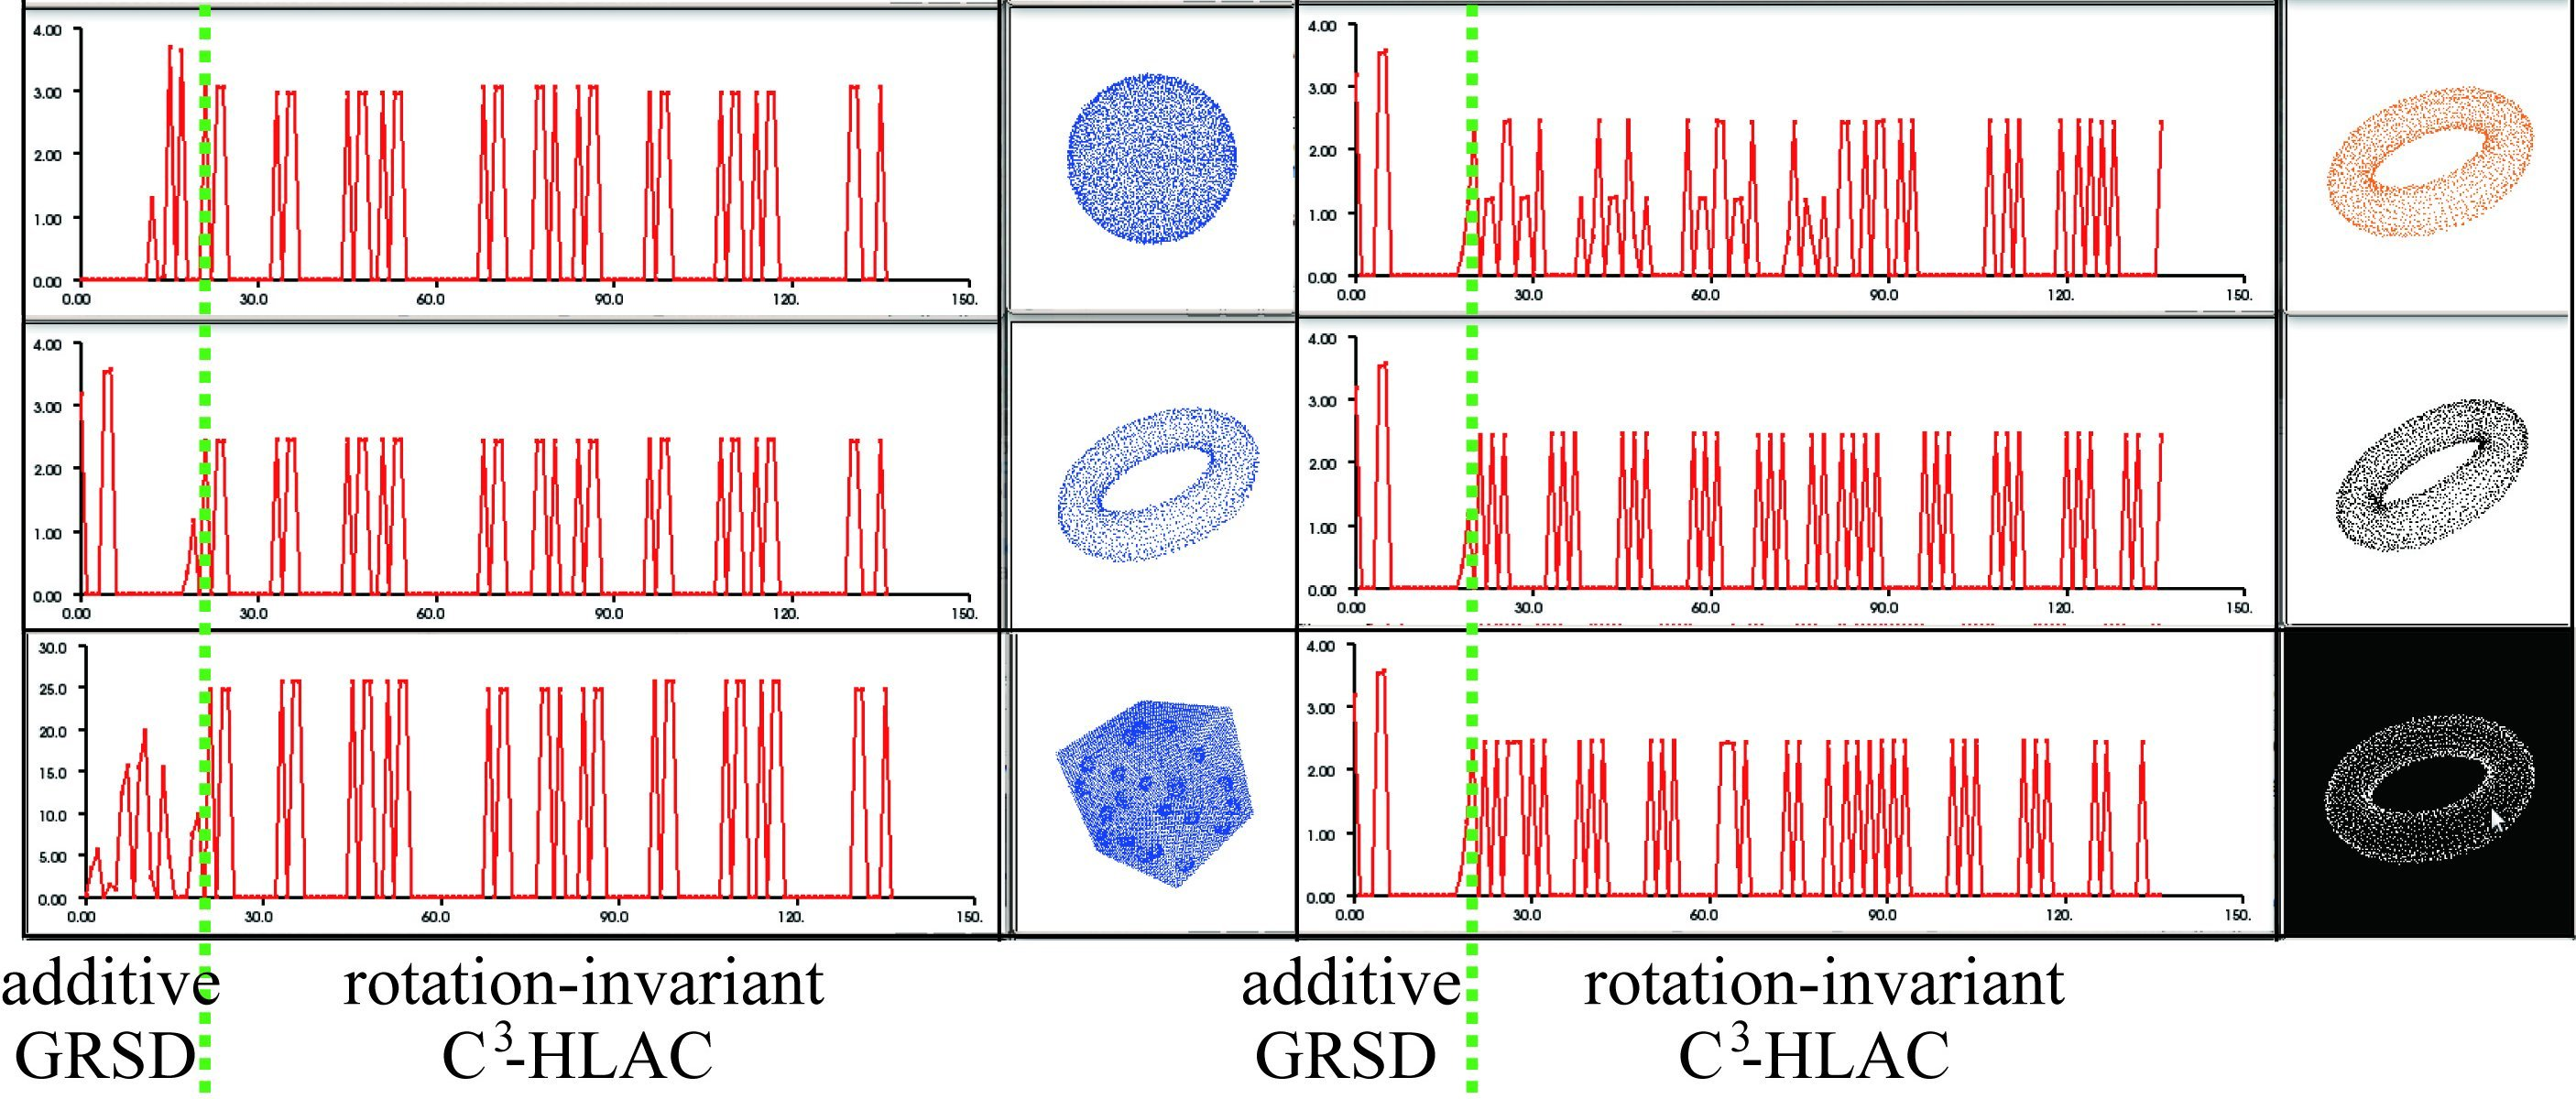
\includegraphics[width=.89\columnwidth]{../figures/colorCHLAC/artificial/normalized_hist_mini.jpg}
  \end{center}
}

\posterboxroundnessstandard
\posterbox[Results]{

  For an exploratory experiment, we ran
  tests on the 7 artificially generated objects with 7 different colors, 
  with 10 different levels of Gaussian noises.

  \begin{center}
  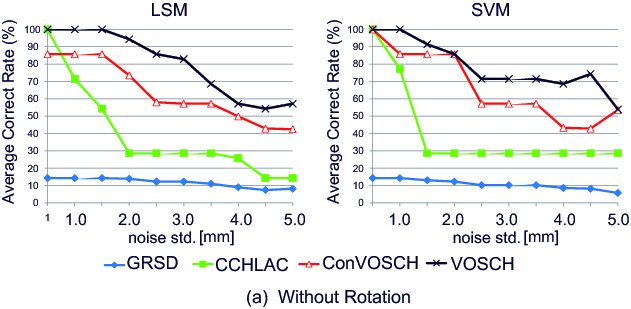
\includegraphics[width=.45\columnwidth]{../figures/synthetic_experiment/synthetic_experimental_result_1.png}
  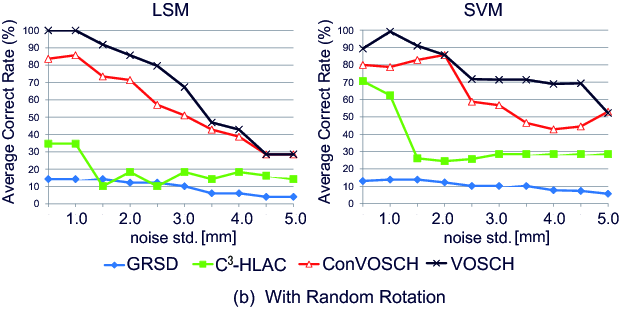
\includegraphics[width=.45\columnwidth]{../figures/synthetic_experiment/synthetic_experimental_result_2.png}
  \end{center}

  \textbf{Accuracy}: \\
  Average correct rate of the classification of 63 objects on novel views was
  30.6\% with GRSD, 68.1\% with C$^3$-HLAC and VOSCH, and \textbf{\emph{72.2\%}} with ConVOSCH.

  \vspace{1ex}

  \textbf{Time}: \\
  Average estimation time needed for an object was \textbf{\emph{0.26 sec.}} \\
  while the average number of points per object was 4632.

  \begin{center}
  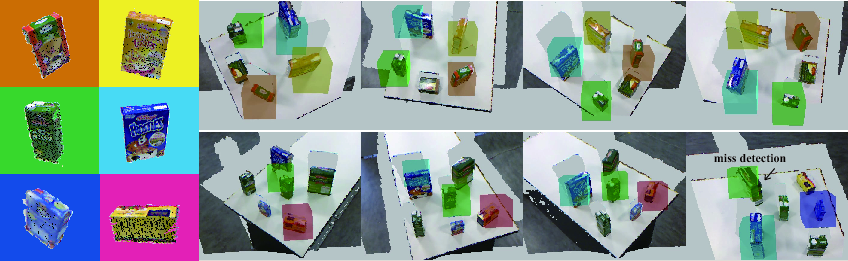
\includegraphics[width=.89\columnwidth]{../figures/detection_demo/four_objects_detection.png}
  \end{center}

}

\posterboxroundnessstandard
\posterbox[Conclusions and Future Work]{

  \begin{itemize}
  \item We presented and evaluated a method to \textbf{\emph{efficiently combine two appearance characteristics 
    into a single feature}} (both rotation variant and rotation invariant).
  \vspace{1ex}
  \item Future work will include the incorporation of other promising 2.5/3D approaches
    into the voxelized feature extraction process.
  \end{itemize}


}

\resizebox{0.9\columnwidth}{!}{
  \begin{minipage}{1.5\columnwidth}
    \bibliographystyle{plain}
    \begin{thebibliography}{1}

    \bibitem{kanezaki2011icra}
      A.~Kanezaki, T.~Suzuki, T.~Harada, and Y.~Kuniyoshi, 
      \newblock {Fast Object Detection for Robots in a Cluttered Indoor Environment Using Integral 3{D} Feature Table},
      \newblock In \emph{Proc. of the IEEE Int. Conf. on Robotics and Automation (ICRA 2011)},
      \newblock 2011.
      %\newblock Shanghai, China: May, 9--13 2011.

    \bibitem{GRSD10Humanoids}
      Z.-C.~Marton, D.~Pangercic, R.~Rusu, A.~Holzbach, and M.~Beetz, 
      \newblock {Hierarchical Object Geometric Categorization and Appearance Classification for Mobile Manipulation},
      \newblock In \emph{Proc. of the IEEE Int. Conf. on Humanoid Robots (Humanoids 2011)},
      \newblock 2010.
      %\newblock Sheraton Nashville Downtown, Nashville, TN: December, 6--8, 2010.

    \end{thebibliography}
  \end{minipage}
}




\end{document}


% \begin{wrapfigure}[14]{r}{0.5\columnwidth}
% \vspace{-1em}
% %\includegraphics[width=0.5\columnwidth]{mapping/objects/CAD/eye-catcher.pdf}
% \end{wrapfigure}
